\documentclass[11pt]{report}

\usepackage[utf8]{inputenc}
\usepackage{mathpazo}
  \renewcommand{\baselinestretch}{1.1}
\usepackage{amssymb}
\usepackage{amsmath}
\usepackage[font={small,it}]{caption}
\usepackage{fancyvrb}
\usepackage[letterpaper, left=1.5in, right=1.5in, top=1in, bottom=1in]{geometry}
\usepackage{hyperref}
  \hypersetup{
    breaklinks=true,
    colorlinks=true,
      anchorcolor=black,
      citecolor=black,
      filecolor=black,
      linkcolor=black,
      urlcolor=black,
    pdftitle={Bayesian Models of Gene Expression and RNA Sequencing},
    pdfauthor={Bob Carpenter, Shuonan Chen, Nikolai Vetr},
    pdfpagemode=FullScreen,
  }
\usepackage{mathtools}
\usepackage[round]{natbib}
\usepackage{sourcecodepro}
\usepackage{tikz}
  \usetikzlibrary{bayesnet,arrows,calc,patterns,positioning,shapes,snakes}
  \tikzstyle{exon}=[draw, minimum size=1.25em, minimum width=3em]
  \tikzstyle{intron}=[draw, mimimum size=1.25em minium width=1.5em, fill=gray!30]
  \tikzstyle{utr}=[exon, fill=blue!30]
  \tikzstyle{utr3}=[exon, fill=blue!30, node distance=3em]
  \tikzstyle{promoter}=[exon, fill=blue!50, minimum width=1em, node distance=2em]
  \tikzstyle{flanking}=[exon, fill=yellow!30]
  \tikzstyle{intron}=[exon, fill=gray!30]
  \tikzstyle{exon1}=[exon, fill=red!30]
  \tikzstyle{exon2}=[exon, fill=red!50]
  \tikzstyle{exon3}=[exon, fill=red!70]
  \tikzstyle{cap5}=[draw, circle, minimum size=1.5em, node distance=2.05em,  fill=orange!30]
  \tikzstyle{capsmall}=[draw, circle, minimum size=0.3em, fill=orange!30]
  \tikzstyle{bead}=[draw, circle, minimum size=1.25em, node distance=1em,  fill=green!30]
  \tikzstyle{rna}=[draw, minimum height=0.1em, minimum width=10em, fill=purple!30]
  \tikzstyle{rnafrag}=[draw, minimum height=0.1em, minimum width=2.5em, fill=purple!30]
  \tikzstyle{dnafrag}=[draw, minimum height=0.1em, minimum width=2.5em, fill=blue!30]
  \tikzstyle{polyA}=[exon, draw=none, fill=white!100, node distance=3.5em]
  \tikzstyle{textbox}=[exon, draw=none, fill=white!100, node distance=4em]
  \tikzstyle{exonB}=[draw, minimum size=0.8em, minimum width=2em]
  \tikzstyle{exon1B}=[exonB, fill=red!50]
  \tikzstyle{exon2B}=[exonB, fill=yellow!50]
  \tikzstyle{exon3B}=[exonB, fill=blue!50]
  \tikzstyle{intronB}=[exonB, fill=gray!30]
  \tikzstyle{splice}=[coordinate, node distance=1.5em]
  \tikzset{%
    body/.style={inner sep=0pt,outer sep=0pt,shape=rectangle,draw,thick,pattern=north east lines wide},
    dimen/.style={<->,>=latex,thin,every rectangle node/.style={fill=white,midway,font=\sffamily}},
    symmetry/.style={dashed,thin},
  }
% \usepackage{tocbibind}
\usepackage{verbatimbox}
\usepackage{xspace}

% basic math
\newcommand{\logit}{\textrm{logit}}
\newcommand{\ilogit}{\logit^{-1}}
\newcommand{\rngto}[1]{1{:}#1}
\newcommand{\setlist}[1]{\{ #1 \}}
\newcommand{\setcomp}[2]{\{ #1 \, : \, #2 \}}
\newcommand{\deriv}[1]{\frac{\textrm{d}}{\textrm{d}#1}}


% constants
\newcommand{\mybase}[1]{\texttt{#1}\xspace}
\newcommand{\baseA}{\mybase{A}}
\newcommand{\baseC}{\mybase{C}}
\newcommand{\baseG}{\mybase{G}}
\newcommand{\baseT}{\mybase{T}}
\newcommand{\baseU}{\mybase{U}}
\newcommand{\baseY}{\mybase{Y}}
\newcommand{\baseN}{\mybase{N}}
\newcommand{\baseR}{\mybase{R}}


% formatting
\newcommand{\stancode}[1]{\verbfilebox[\small]{../../stan/#1}\theverbbox}
\newcommand{\mycaption}[2]{\caption{#2}\label{#1}}
\newcommand{\anitem}[1]{\begin{itemize} \item #1 \end{itemize}}

\setlength{\floatsep}{24pt}

\title{Bayesian Models of Gene Expression and RNA Sequencing}
\author{Bob Carpenter \\ Flatiron Institute
  \and Shuonan Chen \\ Columbia University
  \and Nikolai G.\ Vetr \\ Stanford University}
\date{\the\year-\the\month-\the\day \ (Draft)}

\begin{document}

\maketitle

\begin{abstract}
  \noindent
  We develop a fully Bayesian, generative approach to RNA sequencing
  (RNA-seq) data.  We start with a simple binomial model and
  incrementally expand it to deal with alignment uncertainty, technical
  and biological variation in replicated samples, and differential
  expression among grouped samples.  We introduce multinomial, log, and,
  logistic parameterizations of expected reads and derive the relation
  among multinomial, binomial, Poisson, and negative binomial models of
  read counts. We model expression hierarchically at the group level and
  use partially pooled replicate-level effects to model technical and
  biological variation among replicates.  By treating the alignment of
  multi-aligned reads as a discrete random variable, we can model the
  expression of exons, isoforms, or genes.  Probabilistic inference for
  quantities of interest, such as log fold change between the
  group-level expression of an isoform, follows directly.  We
  demonstrate the robustness of posterior predictive inference in the
  face of limited data, noisy data, and unidentifiable parameters.
\end{abstract}

\tableofcontents

\chapter{Introduction}

We are primarily interested in estimating the relative expression of
genes, exons, or isoforms from RNA sequencing (RNA-seq) data which has
been collected from multiple biologically distinctive groups, with
replicated samples from each group.  The replicates may consist of
multiple cells from a single subject or samples from multiple
subjects.  Our inferential goal is to estimate group-level and
replicate-level expression, from which we can derive probabilities of
differential expression.

Dozens of tools exist to estimate differential expression at the group
level, so it is natural to ask why we are proposing one more.  The
short answer is that almost all of the popular tools that people use
like DESeq2 \citep{love2014differential} or rMATS \citep
{shen2014rmats}, employ heuristic empirical Bayes techniques to
compute an approximate maximum marginal likelihood estimate, followed
by frequentist significance testing for the null hypothesis of no or
small differences in expression.  In contrast, we will present a fully
Bayesian approach that is general enough to encapsulate most of the
models that have been proposed in the literature.

\cite{lewin2019bayesian} provide an excellent overview of Bayesian
differential expression modeling.  Our presentation here is consistent
with theirs, but even more elementary in terms of what it presupposes
of readers in terms of cellular biology or Bayesian statistics.  For
all of the models we discuss, we provide reproducible Stan programs
and R scripts to simulate data and fit models.\footnote{All of our
  code is available from GitHub and open-source licensed. See
  \url{https://github.com/bob-carpenter/BayesExpress}.}


\chapter{DNA, RNA, and Proteins}

We begin with a short overview of RNA sequencing (RNA-seq) technology,
because it will motivate the models we are proposing.  First, we cover
the \textit{in vivo} process of mRNA being transcribed from the genome
and spliced into mRNA.  Second, we describe the \textit{in vitro}
process of enrichment, fragmentation, reverse transcription,
amplification, and sequencing.  The final section describes the
\textit{in silico} process of alignment of the reads to the genome and
expression modeling.

Samples used for RNA-seq may be drawn from a single cell or from a
mixture of cells.  Samples are often organized into groups, such as
wild-type vs.\ cancerous liver cells, or at an even finer grain, with
individual neural cell types.  There are hundreds of human cell types
and cells of a given type change state over time.  In addition, there
is an intrinsic reduction in variability in averaging as shown by the
central limit theorem.  As a result of these two factors, single-cell
RNA-seq data is much more heterogeneous than mixture data.

The process we describe below is a standard one from Illumina, a very
widely used sequencing platform \cite{quail2008large}.  Although we
present a standard process, even the Illumina sequencer allows a wide
range of variation in sample preparation and sequencing used.

\begin{figure}[t!]
  \centering
  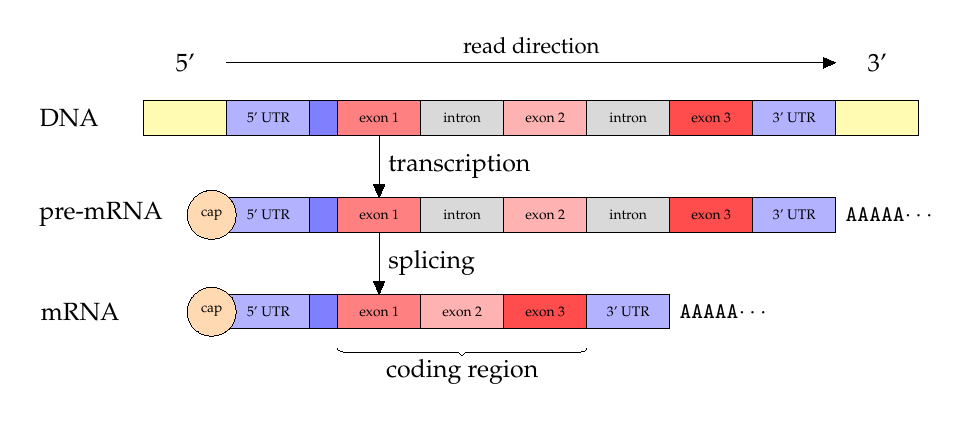
\begin{tikzpicture}[node distance=3em, line width=0mm]
    \node(nc5) [flanking] {};
    \node(utr5) [utr, right of=nc5] {\tiny 5' UTR};
    \node(p) [promoter, right of=utr5] {};
    \node (a1) [exon2, right of=p, node distance=2em] {\tiny exon 1};
    \node (i1) [intron, right of = a1] {\tiny intron};
    \node (a2) [exon1, right of=i1] {\tiny exon 2};
    \node (i2) [intron, right of=a2] {\tiny intron};
    \node (a3) [exon3, right of=i2] {\tiny exon 3};
    \node (utr3) [utr3, right of=a3] {\tiny 3' UTR};
    \node (nc3) [flanking, right of=utr3] {};
    \node (text1) [textbox, left of=nc5, xshift=-0.2em] {\small DNA};
    %
    \node (Butr5) [utr, below of=utr5, node distance=3.5em] {\tiny 5' UTR};
    \node (Bp) [promoter, right of=Butr5] {};
    \node (Ba1) [exon2, right of=Bp, node distance=2em] {\tiny exon 1};
    \node (Bi1) [intron, right of = Ba1] {\tiny intron};
    \node (Ba2) [exon1, right of=Bi1] {\tiny exon 2};
    \node (Bi2) [intron, right of=Ba2] {\tiny intron};
    \node (Ba3) [exon3, right of=Bi2] {\tiny exon 3};
    \node (Butr3) [utr3, right of=Ba3] {\tiny 3' UTR};
    \node (BpolyA) [polyA, right of=Butr3] {\footnotesize \texttt{AAAAA}$\cdots$};
    \node (cap) [cap5, left of=Butr5] {\tiny cap};
    \node (text2) [textbox, left of=cap] {\small pre-mRNA};
    %
    \node (Cutr5) [utr, below of=Butr5, node distance=3.5em] {\tiny 5' UTR};
    \node (Cp) [promoter, right of=Cutr5] {};
    \node (Ca1) [exon2, right of=Cp, node distance=2em] {\tiny exon 1};
    \node (Ca2) [exon1, right of=Ca1] {\tiny exon 2};
    \node (Ca3) [exon3, right of=Ca2] {\tiny exon 3};
    \node (Cutr3) [utr3, right of=Ca3] {\tiny 3' UTR};
    \node (CpolyA) [polyA, right of=Cutr3] {\footnotesize\texttt{AAAAA}$\cdots$};
    \node (Ccap) [cap5, left of=Cutr5] {\tiny cap};
    \node (text2) [textbox, left of=Ccap, xshift=-0.75em] {\small mRNA};

    \node (start5) [textbox, above of=nc5, node distance=2em] {\small 5'};
    \node (end3)  [textbox, above of=nc3, node distance=2em] {\small 3'};
    \draw [->] (start5) -- (end3) node[midway, above] {\footnotesize read direction};
    \draw [->] (a1) -- (Ba1) node[midway, right] {\small transcription};
    \draw [->] (Ba1) -- (Ca1) node[midway, right] {\small splicing};
    \draw [decoration={brace, mirror, raise=0.25cm}, decorate] (Ca1.south west) -- (Ca3.south east)
    node [pos=0.5,anchor=north,yshift=-0.75em] {\small coding region};
  \end{tikzpicture}
  \mycaption{fig:transcriptome-splicing}{Sketch of the \textit{in
      vivo} cellular process that produces mature mRNA through
    transcription and splicing.  DNA (top) is transcribed to pre-mRNA
    (middle); this process starts with the 5' untranslated region
    (UTR) and ends with the 3' UTR.  The dark blue section of the 5'
    UTR indicates the promoter region that is used to regulate the
    transcription process.  After transcription, the pre-mRNA is
    capped on the 5' end and polyadenylated on the 3' end.  The
    introns are then spliced out of the pre-mRNA to form mRNA
    (bottom).  Only the coding region consisting of the exon sequence
    is translated to a sequence of amino acids by the ribosome.}
\end{figure}

\begin{figure}[t!]
  \centering
  \includegraphics[width=2.5in]{../../img/isoform-human-length-histogram.pdf}
  \mycaption{fig:iso-lengths}{Histogram of lengths of the coding
    region of human isoforms, with the $x$-axis on a log scale. The
    transcriptome used is version GRCh38 of the Reference Sequence
    Database Transcripts (RefSeq Transcripts) supplied by the U.S.\
    National Center for Biotechnology Information (NCBI)
    \citep{oleary2016reference}. Only the 80,791 curated isoforms are
    used (i.e., those not marked {\small \texttt{PREDICTED}).}}
\end{figure}

\section{From DNA to mRNA}

A cell's DNA is arranged into chromosomes, each of which consists of a
two strands of nucleotides with opposite orientations arranged in a
double helix. The bases of these nucleotides are adenine (\baseA),
cytosine (\baseC), guanine (\baseG), and thiamine (\baseT). The bases
are attached to an alternating sugar-phosphate backbone which is
oriented with sugar-phosphate bonds at the 5' and 3' atoms of the
sugar ring.

A gene consists of a structured subsequence of bases that begins on
the 5' end with an untranslated region (5' UTR) that is involved in
regulating and initiating a gene's transcription. A gene ends on a 3'
end with a second untranslated region (3' UTR).
\citep{mignone2002untranslated} provide a detailed overview of the
structure and function of the 5' and 3' untranslated regions of a
gene. The central portion of a gene is a sequence of exons separated
by introns. The sketch of the sequence making up a gene is illustrated
in the top line of Figure~\ref{fig:transcriptome-splicing}

During the transcription process, mRNA is transcribed from the DNA,
capped on the 5' end, and polyadenylated on the 3' end with a sequence
of adenine (\baseA) bases known as the poly(A) tail. The resulting
pre-mRNA is shown on the second line of
Figure~\ref{fig:transcriptome-splicing}.

Finally, the introns and possibly some exons are spliced out of the
pre-mRNA to produce the final mRNA, as shown in the bottom line of
Figure~\ref{fig:transcriptome-splicing}. The splicing operation is
often non-deterministic in higher eukaryotes; in humans, most genes
produce multiple splice variants known as isoforms. The final result
of transcription and splicing is mature mRNA, which is then translated
to a polypeptide (i.e., a sequence of amino acids), which then folds
into a protein.

Figure~\ref{fig:iso-lengths} provides a histogram of human isoform
lengths. These lengths vary widely, with the shortest being 33 bases
and the longest 109,224 bases. The median number of bases in an
isoform is 2879, the central 50\% interval is (1714, 4568) and the
central 95\% interval is (100, 10187). The mean isoform length is 3506
and the sample standard deviation is 2856.

We are interested in expression because the genes and isoforms
expressed by a cell determine the cell's function. By studying
differential expression of RNA among cells of different types, we hope
to uncover clues about cell regulation and differentiation.

\section{From mRNA to protein}

\begin{table}[t!]
  \centering\small
  \setlength\doublerulesep{4pt}
  \setlength{\tabcolsep}{4pt}
  \centering\small
  \begin{tabular}{|ccc|c|}
    \hline
    \multicolumn{3}{|c|}{\textit{codon}} & \textit{acid}
    \\ \hline \hline
    \baseU & \baseU & \baseU & phe
    \\ &        & \baseC &
    \\ \hline
    &  & \baseA & leu
    \\ & & \baseG &
    \\ \hline \hline
    \baseC & \baseU & \baseU & leu
    \\ & & \baseC &
    \\ & & \baseA &
    \\ & & \baseG &
    \\ \hline \hline
    \baseA & \baseU & \baseU & ile
    \\ & & \baseC &
    \\ & & \baseA &
    \\ \hline
    &  & \baseG & met$^*$
    \\ \hline \hline
    \baseG & \baseU & \baseU & val
    \\ & & \baseC &
    \\ & & \baseA &
    \\ & & \baseG &
    \\ \hline
  \end{tabular}
  \qquad
  \begin{tabular}{|ccc|c|}
    \hline
    \multicolumn{3}{|c|}{\textit{codon}} & \textit{acid}
    \\ \hline \hline
    \baseU & \baseC & \baseU & ser
    \\ & & \baseC &
    \\ & & \baseA &
    \\ & & \baseG &
    \\ \hline \hline
    \baseC & \baseC & \baseU & pro
    \\ & & \baseC &
    \\ & & \baseA &
    \\ & & \baseG &
    \\ \hline \hline
    \baseA & \baseC & \baseU & thr
    \\ & & \baseC &
    \\ & & \baseA &
    \\ & & \baseG &
    \\ \hline \hline
    \baseG & \baseC & \baseU & ala
    \\ & & \baseC &
    \\ & & \baseA &
    \\ & & \baseG &
    \\ \hline
  \end{tabular}
  \qquad
  \begin{tabular}{|ccc|c|}
    \hline
    \multicolumn{3}{|c|}{\textit{codon}} & \textit{acid}
    \\ \hline \hline
    \baseU & \baseA & \baseU & tyr
    \\ & & \baseC &
    \\ \hline
    &  & \baseA & \textit{stop}
    \\ & & \baseG &
    \\ \hline \hline
    \baseC & \baseA & \baseU & his
    \\ & & \baseC &
    \\ \hline
    &  & \baseA & gln
    \\ & & \baseG &
    \\ \hline \hline
    \baseA & \baseA & \baseU & asp
    \\ & & \baseC &
    \\ \hline
    &  & \baseA & lys
    \\ & & \baseG &
    \\ \hline \hline
    \baseG & \baseA & \baseU & asp
    \\ & & \baseC &
    \\ \hline
    &  & \baseA & glu
    \\ & & \baseG &
    \\ \hline
  \end{tabular}
  \qquad
  \begin{tabular}{|ccc|c|}
    \hline
    \multicolumn{3}{|c|}{\textit{codon}} & \textit{acid}
    \\ \hline \hline
    \baseU & \baseG & \baseU & cys
    \\ & & \baseC &
    \\ \hline
    &  & \baseA & \textit{stop}
    \\ \hline
    &  & \baseG & trp
    \\ \hline \hline
    \baseC & \baseG & \baseU & arg
    \\ & & \baseC &
    \\ & & \baseA &
    \\ & & \baseG &
    \\ \hline \hline
    \baseA & \baseG & \baseU & ser
    \\ & & \baseC &
    \\ \hline
    &  & \baseA & arg
    \\ & & \baseG &
    \\ \hline \hline
    \baseG & \baseG & \baseU & gly
    \\ & & \baseC &
    \\ & & \baseA &
    \\ & & \baseG &
    \\ \hline
  \end{tabular}
  \mycaption{tab:genetic-code}{A figure representing the genetic code,
    which is a mapping from codons consisting of three RNA bases
    (\baseU, \baseC, \baseA, and \baseG) to amino acids and the stop
    signal. The boxes represent the initial two bases, with each row
    sharing the same first base and each column the same second base.
    A single codon encodes tryptophan (trp), whereas six encode
    leucine (leu). The codon \baseA~\baseU~\baseG encodes the amino
    acid methionine (met) and also signals the start of translation. }
\end{table}
%
The ribosome, a molecule composed of ribosomal RNA (rRNA) and
proteins, coordinates the translation of the mRNA to a sequence of
amino acids that will make up a protein. The mRNA is arranged into
groups of three bases, called codons, each of which translates to an
amino acid (one of which does double duty as the start signal), or end
signal. There are 20 distinct amino acids. The genetic code, shown in
Table~\ref{tab:genetic-code}, is the mapping from codons to amino
acids and the stop signal. With $4^3 = 64$ codons and only 20 amino
acids (including one doing double-duty as the start signal) plus the
stop signal, there are cases where more than one codon maps to the
same amino acid. For example, the codons \baseU{}\baseU{}\baseU and
\baseU{}\baseU{}\baseC both translate to the amino acid phenylalanine
(phe), and the codons \baseU{}\baseA{}\baseA, \baseU{}\baseA{}\baseG,
and \baseU{}\baseG{}\baseA all provide a stop signal.

\begin{figure}[t]
  \centering
  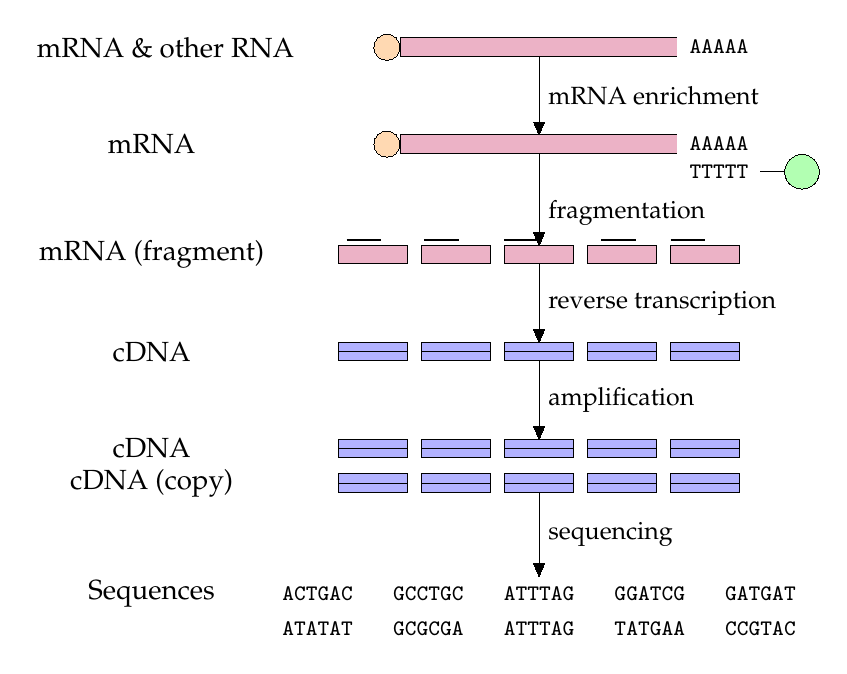
\begin{tikzpicture}[node distance=3em, line width=0mm]
    \node (cap1) [capsmall] {};
    \node (rna1) [rna, right of=cap1, node distance=5.5em] {};
    \node (polyA1) [polyA, right of=rna1, node distance=6.5em] {\footnotesize \texttt{AAAAA}};
    %
    \node (cap2) [capsmall, below of=cap1, yshift=-0.5em] {};
    \node (rna2) [rna, right of=cap2, node distance=5.5em] {};
    \node (polyA2) [polyA, right of=rna2, node distance=6.5em] {\footnotesize \texttt{AAAAA}};
    \node (polyT2) [polyA, below of=polyA2, node distance=1em] {\footnotesize \texttt{TTTTT}};
    \node (bead2) [bead, right of=polyT2, node distance=3em] {};
    \draw [-] (polyT2) -- (bead2) {};
    %
    \node (frag1) [rnafrag, below of=cap2, xshift=-0.5em, yshift=-1em] {};
    \node (frag2) [rnafrag, right of=frag1] {};
    \node (frag3) [rnafrag, right of=frag2] {};
    \node (frag4) [rnafrag, right of=frag3] {};
    \node (frag5) [rnafrag, right of=frag4] {};
    \draw [-, thick] ([yshift=0.2em, xshift=0.3em]frag1.north west) -- ([yshift=0.2em, xshift=0.3em]frag1.north) {};
    \draw [-, thick] ([yshift=0.2em, xshift=0.1em]frag2.north west) -- ([yshift=0.2em, xshift=0.1em]frag2.north) {};
    \draw [-, thick] ([yshift=0.2em]frag3.north west) -- ([yshift=0.2em]frag3.north) {};
    \draw [-, thick] ([yshift=0.2em, xshift=0.5em]frag4.north west) -- ([yshift=0.2em, xshift=0.5em]frag4.north) {};
    \draw [-, thick] ([yshift=0.2em]frag5.north west) -- ([yshift=0.2em]frag5.north) {};
    %
    \node (dna1) [dnafrag, below of=frag1, yshift=-0.5em] {};
    \draw [-] (dna1.west) -- (dna1.east) {};
    \node (dna2) [dnafrag, right of=dna1] {};
    \draw [-] (dna2.west) -- (dna2.east) {};
    \node (dna3) [dnafrag, right of=dna2] {};
    \draw [-] (dna3.west) -- (dna3.east) {};
    \node (dna4) [dnafrag, right of=dna3] {};
    \draw [-] (dna4.west) -- (dna4.east) {};
    \node (dna5) [dnafrag, right of=dna4] {};
    \draw [-] (dna5.west) -- (dna5.east) {};
    %
    \node (dna1b) [dnafrag, below of=dna1, yshift=-0.5em] {};
    \draw [-] (dna1b.west) -- (dna1b.east) {};
    \node (dna2b) [dnafrag, right of=dna1b] {};
    \draw [-] (dna2b.west) -- (dna2b.east) {};
    \node (dna3b) [dnafrag, right of=dna2b] {};
    \draw [-] (dna3b.west) -- (dna3b.east) {};
    \node (dna4b) [dnafrag, right of=dna3b] {};
    \draw [-] (dna4b.west) -- (dna4b.east) {};
    \node (dna5b) [dnafrag, right of=dna4b] {};
    \draw [-] (dna5b.west) -- (dna5b.east) {};
    %
    \node (dna1c) [dnafrag, below of=dna1b, yshift=1.75em] {};
    \draw [-] (dna1c.west) -- (dna1c.east) {};
    \node (dna2c) [dnafrag, right of=dna1c] {};
    \draw [-] (dna2c.west) -- (dna2c.east) {};
    \node (dna3c) [dnafrag, right of=dna2c] {};
    \draw [-] (dna3c.west) -- (dna3c.east) {};
    \node (dna4c) [dnafrag, right of=dna3c] {};
    \draw [-] (dna4c.west) -- (dna4c.east) {};
    \node (dna5c) [dnafrag, right of=dna4c] {};
    \draw [-] (dna5c.west) -- (dna5c.east) {};
    %
    \node (seq3) [textbox, below of=dna3c] {\footnotesize\tt ATTTAG};
    \node (seq4) [textbox, right of=seq3] {\footnotesize\tt GGATCG};
    \node (seq5) [textbox, right of=seq4] {\footnotesize\tt GATGAT};
    \node (seq2) [textbox, left of=seq3] {\footnotesize\tt GCCTGC};
    \node (seq1) [textbox, left of=seq2] {\footnotesize\tt ACTGAC};
    %
    \node (seq3b) [textbox, below of=seq3, yshift=2.75em] {\footnotesize\tt ATTTAG};
    \node (seq4b) [textbox, right of=seq3b] {\footnotesize\tt TATGAA};
    \node (seq5b) [textbox, right of=seq4b] {\footnotesize\tt CCGTAC};
    \node (seq2b) [textbox, left of=seq3b] {\footnotesize\tt GCGCGA};
    \node (seq1b) [textbox, left of=seq2b] {\footnotesize\tt ATATAT};

    \node (label1) [textbox, left of=seq3, xshift=-10em] {Sequences};
    \node (label2) [textbox, left of=dna1c, xshift=-4em] {cDNA (copy)};
    \node (label3) [textbox, left of=dna1b, xshift=-4em] {cDNA};
    \node (label4) [textbox, left of=dna1, xshift=-4em] {cDNA};
    \node (label5) [textbox, left of=frag1, xshift=-4em] {mRNA (fragment)};
    \node (label6) [textbox, left of=cap2, xshift=-4.5em] {mRNA};
    \node (label7) [textbox, left of=cap1, xshift=-4em] {mRNA \& other RNA};
    %
    \draw [->] (rna1) -- (rna2) node[midway, right] {\small mRNA enrichment};
    \draw [->] (rna2) -- (frag3) node[midway, right, yshift=-0.5em] {\small fragmentation};
    \draw [->] (frag3) -- (dna3) node[midway, right] {\small reverse transcription};
    \draw [->] (dna3) -- (dna3b) node[midway, right] {\small amplification};
    \draw [->] (dna3c) -- (seq3) node[midway, right] {\small sequencing};
  \end{tikzpicture}
  \mycaption{fig:cDNA-synthesis}{Sketch of the \emph{in vitro} laboratory process for a typical RNA sequencing experiment.  The first step, poly(A) selection, uses magnetic beads to bind to the poly(A) tails of mRNA to enrich it relative to other RNA such as ribosomal RNA (rRNA) or microRNA (miRNA).  The second step, fragmentation by random hexamers, introduces random short oligo-DNA sequences that anneal at multiple points along the mRNA transcript and serve as primers for reverse transcription.  Reverse transcription synthesizes double-stranded cDNA from the mRNA fragments.  These double-stranded cDNA fragments are then amplified with a polymerase chain reaction (PCR).  In the final step, the sequencer ``reads'' the bases of the cDNA fragments and reports them as a sequence of characters.}
\end{figure}

\chapter{RNA Sequencing \& Alignment}

\section{Reverse transcription and sequencing}

Because sequencers work on short sequences of double-stranded cDNA, an
mRNA sample must be fragmented and reverse transcribed before
sequencing. To filter a biological sample to the mRNA to reverse
transcribe, either the the poly(A) tails of mRNA are selected or the
ribosomic RNA is depleted from the sample. The remaining mRNA is then
fragmented and then primed for reverse transcription using either
oligo(dT) priming or random hexamer primers. Oligo(dT) priming is
heavily biased toward the 3' end of the mRNA because it binds to the
poly(A) tail of mRNA. Random hexamers are biased to such an extent
that initial hexamer counts can vary by an two orders of magnitude.
The primed mRNA is then reverse transcribed to cDNA.

After being reverse transcribed from the mRNA fragments, the
synthesized cDNA is sequenced. The Illumina sequencing process is
based on imaging of complementary nucleotides tagged with fluorescent
markers. Imaging software then makes the call as to which base was
present on the cDNA. For short single reads on the order of 100 bases,
the Illumina sequencing process has 99\% or more accuracy per base,
with accuracy declining along the sequence~\citep{tan2019long}.

Most sequencing technologies produces reads on the order of 100 bases
long. Long-read sequencing (LRS) technology, such as single-molecule
real-time sequencing \citep{ardui2018single} from Pacific Biosciences
and nanopore sequencing from Oxford Nanopores Technology
\citep{deamer2016three}, can sequence up to 10,000 bases. These bases
require an entirely different paradigm of analysis due to higher error
rates and the fact that most mRNA is shorter than 10,000 bases. In
addition to a higher error rate, long-read sequencing has lower
throughput and requires fresh samples to avoid mRNA degradation
\citep{mantere2019long}.

\section{Alignment}

For all of the analyses we discuss here, we will assume that a
reference genome sequence or transcriptome sequence is available. A
reference genome is a set of reference chromosomes, each of which is
represented as a sequence of bases including genes and other genetic
material, with the genes being further subdivided into a sequence of
exons and introns. A reference transcriptome is a set of reference
isoforms, each of which consists of a sequence of exons.

\begin{table}[t!]
  \centering\small
  \begin{tabular}{r|cccccccccccccc}
    \textit{read} &  & & & \baseA & \baseG & \baseT & \baseT & \baseC & \baseA & \baseG &
    \\
    \textit{reference} & $\cdots$ & $\cdots$ & \baseG & \baseA & \baseG & \baseT & \baseT & \baseC & \baseA & \baseG & \baseG & $\cdots$ & $\cdots$
    \\ \hline
    \textit{exons} & $\cdots$ & \multicolumn{11}{|c|}{exon 1} & $\cdots$
  \end{tabular}
  \\[12pt]
  \begin{tabular}{r|ccccccccccccccc}
    \textit{read} &  & & & \baseA & \baseG & \baseT & & \baseT & \baseC & \baseA & \baseG &
    \\
    \textit{reference} & $\cdots$ & $\cdots$ & \baseG & \baseA & \baseG & \baseT & $\cdots$ & \baseT & \baseC & \baseA & \baseG & \baseG & $\cdots$ & $\cdots$
    \\ \hline
    \textit{exons} & $\cdots$ & \multicolumn{5}{|c|}{exon 1} & intron
                         & \multicolumn{6}{|c|}{exon 2}
  \end{tabular}
  \\[12pt]
  \begin{tabular}{r|ccccccccccccccc}
    \textit{read} &  & & & \baseA & \baseG & \baseT & \baseT & \baseC & \baseA & \baseG &
    \\
    \textit{reference} & $\cdots$ & $\cdots$ & \baseG & \baseA & \baseG & \baseT & \baseT & \baseC & \baseA & \baseG & \baseG  & $\cdots$ & $\cdots$
    \\ \hline
    \textit{exons} & $\cdots$ & \multicolumn{5}{|c|}{exon 1}
                       & \multicolumn{6}{|c|}{exon 2}
  \end{tabular}
  \mycaption{tab:split-align}{Examples of aligning mRNA reads to the
    genome and transcriptome. Reads may align to the genome or
    transcriptome fully within an exon (top). Alignments of reads to
    the genome may cross exon junctions (middle). Alignment of
    cross-exon reads to the transcriptome does not require splitting
    (bottom).}
  \label{tab:my_label}
\end{table}

The first step of \textit{in silico} analysis is to align each read,
consisting of a short sequence of called bases, to a reference genome
or reference transcriptome. When aligning to the genome, mRNA
fragments may cross exon junctions, which complicates genome alignment
algorithms and results. Alignment to the transcriptome does not
require splitting the reads, but ambiguous reads are much more
prevalent due to repeated sequences of exons across isoforms.
Table~\ref{tab:split-align} illustrates alignments within and across
exons in the genome and transcriptome.

The bases in a reference genome or transcriptomes are merely a sketch,
known as a consensus sequence, of what an individual's genome might
look like. Human genomes vary at a rate of roughly one base per
thousand, with most variation being in the form of single nucleotide
polymorphisms (SNPs), which involve the substitution, insertion, or
deletion of a single base. Table~\ref{tab:edit-distance} shows example
alignments involving a single substitution, deletion, or insertion.

\begin{table}[t!]
  \centering
  \begin{tabular}{c|c|c}
    \textit{type} & \textit{effect} & \textit{example}
    \\ \hline
    synonymous & same amino acid & \baseU{}\baseU{}\baseU $\rightarrow$ \baseU{}\baseU{}\baseC
    \\
                  & & \baseU{}\baseU{}\baseA{} $\rightarrow$ \baseC{}\baseU{}\baseA
    \\ \hline
    missense & different amino acid & \baseC{}\baseA{}\baseU $\rightarrow$ \baseC{}\baseA{}\baseA
    \\
                  & & \baseC{}\baseA{}\baseU $\rightarrow$ \baseC{}\baseC{}\baseU
    \\
                  & & \baseC{}\baseA{}\baseU $\rightarrow$ \baseG{}\baseA{}\baseU
    \\ \hline
    nonsense & stop signal & \baseC{}\baseA{}\baseA{} $\rightarrow$ \baseU{}\baseA{}\baseA{}
    \\
                  & & \baseU{}\baseC{}\baseA $\rightarrow$ \baseU{}\baseG{}\baseA
    \\
                  & & \baseU{}\baseA{}\baseC $\rightarrow$ \baseU{}\baseA{}\baseG
  \end{tabular}
  \mycaption{tab:snp-types}{There are three possible effects of a singular nucleotide polymorphism.}
\end{table}

Substitution of bases within a codon have three different types of
effects. A synonymous substitution is one in which the amino acid
being coded does not change. For example, \baseU{}\baseC{}\baseU and
\baseU{}\baseC{}\baseA both code for serine, so substituting \baseU
for \baseA in the third position of a codon beginning with
\baseU{}\baseC is an example of a synonymous substitution. Synonymous
substitutions may nevertheless cause differences in expression because
of differences in translation efficiency. A missense substitution
causes the wrong amino acid to be coded. For example, because
\baseU\baseU\baseU codes phenylalanine and \baseU{}\baseC{}\baseU
codes serine, substituting \baseU for \baseC in the second position
here results in a missense substitution. A nonsense substitution turns
a codon that codes for an amino acid into a stop codon. For instance,
\baseC{}\baseA{}\baseA codes for glutamine (gln), whereas
\baseU{}\baseA{}\baseA is the stop codon, so a substitution of \baseU
for \baseC in the first position of a codon ending in \baseA{}\baseA
results in a nonsense substitution.

\begin{table}[t!]
  \centering\small
  \begin{tabular}{r|cccccccccccl}
    \textit{read} & & \baseG & \baseA & \baseG & \baseT & \baseT & \baseC & \baseA & \baseG
    \\
    \textit{reference} & $\cdots$ & \baseG & \baseA & \baseG & \baseC & \baseT & \baseC & \baseA & \baseG & $\cdots$
    \\ \hline
    \textit{edits} &  & - & - & - & \small S & - & - & - & - &  & \small (distance 1, substitute)
  \end{tabular}
  \\[12pt]
  \begin{tabular}{r|ccccccccccccl}
    \textit{read} & & \baseG & \baseA &\baseT & \baseG & \baseT & \baseT & \baseC & \baseA & \baseG &
    \\
    \textit{reference} & $\cdots$ & \baseG & \baseA & \baseT & \baseG & \baseT & \baseT & \baseC & $\bullet$ & \baseG & $\cdots$
    \\ \hline
    \textit{edits} & & - & - & - & - & - & - & - & \small I & - & & \small (distance 1, insert)
  \end{tabular}
  \\[12pt]
  \begin{tabular}{r|ccccccccccccl}
<    \textit{read} & & \baseG & $\bullet$ & \baseC & \baseG & \baseT & \baseT & \baseC & \baseA & \baseG &
    \\
    \textit{reference} & $\cdots$ & \baseG & \baseA & $\baseC$ & \baseG & \baseT & \baseT & \baseC & \baseA & \baseG & $\cdots$
    \\ \hline
    \textit{edits} & & - & \small D & - & - & - & - & - & - & - & & \small (distance 1, delete)
  \end{tabular}
  \mycaption{tab:edit-distance}{Examples of alignments of reads to
    reference genome or transcriptome with a single nucleotide
    polymorphism (SNP). S represents substitution, I insertion, and D
    deletion. A bullet is used to signal the point of insertion in the
    reference or the point of deletion in the read. Alignments can
    potentially have any number of edits, but are typically restricted
    to an edit distance threshold of 1 or 2.}
\end{table}

With the combination of calling errors by the sequencers and the SNPs
in the individuals being sequenced relative to any reference genome or
transcriptome, we typically allow alignment to be inexact and contain
some number of insertions, deletions, or substitutions of bases as
part of the alignment. Allowing inexact matches exacerbates the
multiple alignment problem in both genome and transcriptome alignment.
To reduce computational burden and to simplify statistical analysis,
practitioners often keep only the alignments that have minimal number
of (weighted) edits and sometimes even discard an entire read if there
is not a unique closest alignment.

Another complicating factor in alignment is that the natural 5' to 3'
orientation of the fragments is lost during sequencing. Therefore,
aligners try to align both directions of a fragment to target
sequences. Sometimes, RNA transcription goes wrong and a read is
generated in the 3' to 5' direction, producing an antisense read.
\cite{mourao2019detection} discuss how to correct for potential biases
due to antisense reads using strand-specific RNA-seq.

A major complication with alignment is that a short sequence of bases
may align to more than one location on the genome. Although it would
be possible for each 50-base sequence to be unique (there are $4^{50}$
of them, an astronomically large number), there are motifs that are
repeated across genes.


\chapter{Data Format}

Choosing the format of data we wish to deal with and how we
characterize it mathematically will determine the kinds of models we
can build. We focus on RNA-seq data that has been aligned to a
reference transcriptome or to the exons and exon junctions in a
reference genome. We will use long-form data tables for their
flexibility as well as compatibility with tools such as R and Python.

Because there are typically billions of mRNA sequences being aligned
and millions of alignment targets in a transcriptome, representing
alignments as sufficient statistics at the isoform or genome level can
compress data by several orders of magnitude. Although we have only
discussed single reads, one nice aspect of using sufficient statistics
is that the same models will apply to paired-end reads once they are
reduced to target alignments.


\section{Experimental design}

RNA sequencing data consists of a set of biological samples arranged
into groups representing one or more distinct biological conditions.
Within a group, the samples may represent biological replicates (e.g.,
tissue from multiple organisms or multiple cells within an organism)
or technical replicates (e.g., multiple sequencing runs of the same
sample). The experimental design is determined by the number of groups
in the experiment and the number of samples in each group, as well as
the number of reads to be extracted from each sample.  

\begin{table}[t!]
  \centering
  \begin{tabular}{|c|c|}
    \multicolumn{2}{c}{group for sample} \vspace*{2pt} \\ \hline
    \textit{sample} & \textit{group}
    \\ \hline
    \footnotesize $\rngto{S}$ & \footnotesize $\rngto{G}$
    \\
    \footnotesize (index) &
    \\ \hline \hline
    $\vdots$ & $\vdots$
    \\ \hline
  \end{tabular}
  %
  \qquad
  %
  \begin{tabular}{|c|c|}
    \multicolumn{2}{c}{sample for read} \vspace*{2pt}
    \\ \hline
    \textit{read} & \textit{sample}
    \\ \hline
    \footnotesize $\rngto{N}$ & \footnotesize $\rngto{S}$
    \\
    \footnotesize (index) & \footnotesize
    \\ \hline \hline
    $\vdots$ & $\vdots$
    \\ \hline
  \end{tabular}
  %
  \\[9pt]
  %
  \begin{tabular}{|c|c|c|}
    \multicolumn{3}{c}{read alignment} \vspace*{2pt} \\ \hline
    \textit{read} & \textit{target} & \textit{score} \\ \hline
    \footnotesize $\rngto{N}$ & \footnotesize $\rngto{T}$ & \footnotesize {\sc float} \\
    \footnotesize (multi-index) & &
    \\ \hline \hline
    $\vdots$ & $\vdots$ & $\vdots$
    \\ \hline
  \end{tabular}
  \mycaption{tab:rna-seq-data}{Database schema for target-aligned RNA
    sequencing data. The first table (top left) associates samples
    with their groups. The second table (top right) assigns reads to
    their sample. The alignments are provided in the third table
    (bottom). Each alignment comes with a real-valued score, which is
    rendered as a floating-point number. In the sample and read
    tables, the first column is a unique index.  In the read alignment
    table, a read may appearin more than one row, so the index is not
    unique.} \end{table}

\section{Relational representation}

Although storage might be a few CSV files or a shared database,
conceptually, our data is relational.  This section describes its
relational format.

\subsection{Grouping of samples}

Suppose that we have a number of samples and groups, and a function
mapping each sample to its group.
%
\begin{itemize}
\item $S \in \mathbb{N}$ is the number of samples,
\item $G \in \mathbb{N}$ is the number of groups, and
\item $\textrm{group}_s \in \rngto{G}$ is the group to which sample $s \in \rngto{S}$ belongs.
\end{itemize}
%
The database schema for the grouping of samples is given in the top
left of Table~\ref{tab:rna-seq-data}.  There is only one group for
each sample, so the index is unique.  

\subsection{Reads by sample}

Mathematically, we can index all of the reads in our experiment and
assume there is a function mapping the reads to the sample from which
they were drawn.
%
\begin{itemize}
\item $N \in \mathbb{N}$ is the number of RNA sequence reads, and
\item $\textrm{sample}_n \in \rngto{S}$ is the sample from which read
  $n \in \rngto{N}$ is drawn. 
\end{itemize}
%
The read provenance is represented as a database table, the schema for
which is displayed in the upper right of Table~\ref{tab:rna-seq-data}.
The function from read to sample is unique, so the index on the read
coliumn is unique.  The reverse mapping is not unique, but there may
still be an index to efficiently return the reads in a sample.

\subsection{Read alignment to targets}

Reads will be aligned to genome or transcriptome targets of interest.
An alignment target might represent (a) a gene, (b) an isoform of a
gene, or (c) a single exon or exon junction, (d) pairs of exons and
exon and exon junctions, or (e) ribosomic and micro-RNA transcripts.
Depending on the distance threshold for alignments and how they are
filtered, a read may align to more than one target. These target
alignments are aggregated from the primitive genome-level or
transcriptome-level alignments.

In the database table, each read and target pair is assigned a score.
Because we are working in probabilistic models, we will generally
assume the score for a read/target pair is the log probability that
of a random read from the specified target being the specified read.
We need a new constant for the number of targets, plus a relation
between reads and the targets to which they align.
%
\begin{itemize}
\item $T \in \mathbb{N}$ is the number of alignment targets, and
\item $\log p(\textrm{read}_n \mid \textrm{target} = t) \leq 0$
  is the log probability of the read given the target.
\end{itemize}
This probability may take into account hexamer biases, positional
biases, etc.  In our subsequent models, we will assume it does not
take into account read quality.  

The relational schema for the aligned reads is shown in the bottom row
of Table~\ref{tab:rna-seq-data}.


\chapter{The Master Model}

Like a master recipe, which may be adapted to different ingredients,
the master model for RNA sequencing is a generative model of how reads
are produced, which may be adapted to a wide variety of
parameterizations, priors, and experimental designs.  The master model
generates reads by first selecting an isoform according to the
distribution of isoforms in the sample, and then generating the read
itself according to the probability of reads in the selected isoform.

\section{Sample composition of isoforms}

Suppose there is a total of $N$ reads targeting $T$ distinct isoforms.
Our parameter of interest is a simplex $\theta \in \bigtriangleup\!^T$
denoting the expected composition of our sample.\footnote{The set
  $\bigtriangleup\!^T$ of $T$-simplexes is defined by
  \[
    \bigtriangleup\!^T
    = \{ \theta \in \mathbb{R}^T : 
    \textrm{sum}(\theta) = 1
    \ \textrm{and} \
    \theta_t \geq 0 \ \textrm{for all} \ t \in \rngto{T}
    \}.
  \]
}
Let
$z_n \in \rngto{T}$ be the isoform from which read $n \in \rngto{N}$
originates. The basic assumption of the master model is that the reads
are independent and distributed as
\[
  z_n \sim \textrm{Categorical}(\theta).
\]
The simplex $\theta$ represents proportion of reads that arise from
each isoform, which due to biases involved in the laboratory process,
is typically not the same as the proportion of isoforms.  One of the
ways in which we will consider modifying the master model is by
reparametrizing in terms of isoform proportion using estimates of the
laboratory biases, which allows priors to be expressed on their
natural scale.

\section{Isoform composition of reads}

Given an isoform source $z_n$, read $n$ will be generated according to
an isoform-specific simplex $\phi_t$ denoting the probability of a
given read arising from isoform $t$.  The explicit dimensionality of
the reads and hence $\phi_t$ is astronomical (e.g., $4^{50}$ for 50~bp
reads).  For any given isoform $t$, the distribution $\phi_t$ over
possible reads will be sparse with a size determined by the number of
reads $L_t$ that may arise from isoform $t$.  Read $n$ is then drawn
categorically from the distribution of reads for the isoform $t = z_n$
from which it arose,
\[
  r_n \sim \textrm{Categorical}(\phi_{z_n}), 
\]

\section{Master model likelihood}

The source isoform $z_n$ of read $n$ may be treated as a kind of
missing data.  From this angle, the master model is a mixture over
isoforms.  

\subsection{Complete data likelihood}

The complete data likelihood is derived from the independence
assumption over reads as
\[
  p(r, z \mid \theta, \phi)
  = \prod_{n=1}^N p(r_n, z_n \mid \theta, \phi),
\]
where the complete data likelihood for a given read and its source are
as defined above for the master model,
\[
  p(r_n, z_n \mid \theta, \phi)
  = \textrm{Categorical}(z_n \mid \theta)
  \cdot \textrm{Categorical}(r_n \mid \phi_{z_n}).
\]

\subsection{Observed Data likelihood}

The complete data likelihood cannot be used directly because $z_n$ is
not observed.  One approach might be to estimate the $z_n$ through
sampling, but sampling discrete variables is a combinatorial problem
which can often be slow or even intractable.  Instead, the standard
approach is to marginalize out the missing data to derive the
likelihood of the observed data, which is just the likelihood.  This
is achived by unfolding the likelihood using our independence
assumption,
\[
  p(r \mid \theta, \phi)
  = \prod_{n=1}^N p(r_n \mid \theta, \phi),
\]
and then marginalizing the complete data likelihood for a single read,
\begin{eqnarray*}
  p(r_n \mid \theta, \phi)
  & = & \textstyle \sum_{t=1}^T p(r_n, z_n = t \mid \theta, \phi)
  \\[4pt]
  & = & \textstyle \sum_{t=1}^T p(z_n = t \mid \theta) \, p(r_n \mid \phi_t)
  \\[4pt]
  & = & \textstyle \sum_{t=1}^T \textrm{Categorical}(t \mid \theta)
        \cdot \textrm{Categorical}(r_n \mid \phi_t).
\end{eqnarray*}

\section{Variations of the master model}

Belowm, we will consider a number of specializations and embeddings of
the master model.  For example, we might have data where the $z_n$ are
observed in the sense of being derived from alignments.  

We also consider varations in which $z_n$
is known to fall in a small subset, as we might know after performing
fast $k$-mer level alignment.

Hierarchical models arise by consider a number of samples and joining
the priors for expression, allowing partial pooling, also known as
sharing strength.

Overdispersion due to technical or biological variation may be modeled
by assuming a random effect for each replicate.  The resulting
expression is marginally negative binomial for each isoform.


\chapter{Distinctively Aligned Reads}

We first consider models where every read is aligned to one and only
one target isoform (or gene). The simplicity of such models makes them
easy to understand and perform inference for. They are thus popular in
the literature, being deployed in systems such as rMATS
\citep{shen2014rmats}.

Even with such simple models, we will be able to explore a variety of
topics, including length normalization and read bias, parameterization
of proportions, and how to compare expression levels using Bayesian
posterior predictive inference.


\section{Beta-binomial: proportion spliced in}

We will build up a sequence of increasingly rich Bayesian models
starting with a straightforward binomial model of cassette exon
splicing. A cassette exon is a single exon that is alternatively
included or spliced out of isoforms.

For any given cassette exon, there may be more than one isoform that
includes it and more than one isoform that excludes it. Rather than
modeling the expression of individual isoforms, we restrict attention
to whether the exon is included or excluded. Our quantity of interest
is the proportion of transcripts in which the exon is included,
$\psi \in [0, 1]$, which is known as the percent spliced in index
(PSI).%
\footnote{Genomics has adopted several non-unitary units.
  Rather than walking back percentage units using ``index'', it would
  have been simpler to call $\psi$ the ``proportion spliced in.''}

\begin{figure}[t!]
  \centering
  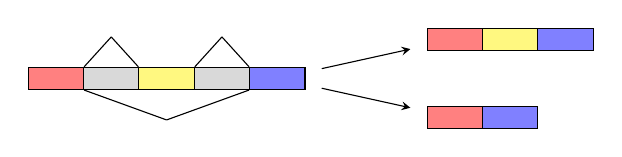
\begin{tikzpicture}[node distance=2em]
    \node (a) [exon1B] {};
    \node (i1) [intronB, right of=a] {};
    \node (b) [exon2B] [right of=i1] {};
    \node (i2) [intronB, right of=b] {};
    \node (c) [exon3B] [right of=i2] {};
    \node (sp) [coordinate, node distance=5em, right of=c] {};
    %
    \node (iso1) [splice, above of=i1] {};
    \draw [black] (a.north east) -- (iso1);
    \draw [black] (iso1) -- (b.north west);
    \node (iso2) [splice, above of=i2] {};
    \draw [black] (b.north east) -- (iso2);
    \draw [black] (iso2) -- (c.north west);
    %
    \node (iso3) [splice, below of=b] {};
    \draw [black] (a.south east) -- (iso3);
    \draw [black] (iso3) -- (c.south west);
    %
    \node (a1) [exon1B, above right of=sp] {};
    \node (b1) [exon2B, right of=a1] {};
    \node (c1) [exon3B, right of=b1] {};
    \path[->, >=stealth, shorten >= 6pt, shorten <= 6pt] (c) edge node {} (a1);
    %
    \node (a2) [exon1B, below right of=sp] {};
    \node (c2) [exon3B, right of=a2] {};
    \path[->, >=stealth, shorten >= 6pt, shorten <= 6pt] (c) edge node {} (a2);
  \end{tikzpicture}
  \mycaption{fig:cassette-exon}{The pre-mRNA (left) undergoes
    splicing, with the cassette exon (yellow) either included (right,
    top) or excluded (right, bottom). The base of the back triangles
    above and below the genome sequence (left) indicates material that
    is spliced out. In the inclusion case (top), only the two introns
    (grey) are spliced out.  In the exclusion case (bottom), both
    introns and the middle exon are spliced out. Distinctive reads for
    inclusion are those in the casette exon or crossing its 5'
    junction (red--yellow) or 3' junction (yellow--blue); distinctive
    reads for exclusion are those crossing the splice junction (red--blue).}
\end{figure}

Figure~\ref{fig:cassette-exon} shows a genetic sequence composed of
three exons separated by introns, along with two choices for splicing,
one with and one without the cassette exon.

In this first example, we will restrict ourselves to a single RNA-seq
sample ($S = 1$), which entails a single group ($G = 1$). This lets us
just ignore sample and group structure for the time being. We will
further restrict attention to distinctive reads, meaning reads that
occur in the spliced-in variant or the spliced-out variant, but not
both. A distinctive read indicates splicing in if it falls entirely
within the cassette exon or crosses its junctions with other exons; a
read indicates splicing out if it is drawn from the junction excluding
the cassette exon.

Although not likely given our read lengths, it is technically possible
for a read to align within the cassette exon or on one of its
junctions and also lie on the junction of the excluded cassette exon.
Such non-distinctive reads are excluded from consideration.

On the other hand, we can retain reads that align non-uniquely within
the splicing-in case as long as they cannot be aligned across the
splicing-out junction. Similarly, we can retain reads that align in
more than one way across the splicing-out junction if they cannot be
aligned within the cassette exon or across its junctions. The key
consideration is that however we filter reads, we need to adjust $L_t$
to be the number of possible read positions in isoform $t$, taking
into account the filtering process.

\subsection{Data}

We are going to need to adjust read probabilities by the number of
possible targets.  Let
%
\begin{itemize}
\item $L_t$ be the number of positions in target $t$ with distinctive
  reads for target $t$.
\end{itemize}
%
In the cassette exon example, $L_1$ is the number of reads that can
align within the cassette exon or crossing one of its splice junction
and $L_2$ is the number of reads that cross the junction splicing out
the cassette exon. The sizes of these sets will depend on the size of
the cassette exon and the length of the reads.

Here we have two targets, $T = 2$, with $t = 1$ being the inclusion
case and $t = 2$ the exclusion case.  We will assume our data has been
filtered for alignment and read quality.  We will assume
%
\begin{itemize}
\item $N \in \mathbb{N}$ is the total number of distinctive reads for
  the cassette exon, and
\item $y \in 0{:}N$ is the number of distinctive reads aligning within
  the cassette exon or across its splice junctions.
\end{itemize}

\subsection{Likelihood}

We will use a very simple parameterization, with a single variable
%
\begin{itemize}
\item $\psi \in (0, 1)$, the proportion of transcripts with the
  cassette exon included.
\end{itemize}
%
With this transcript composition, the number of reads we expect to see
that include the cassette exons should be proportional to $L_1 \cdot
\psi$, with the number of reads that exclude the cassette exon being
proportional to $L_2 \cdot (1 - \psi)$.  This allows us to
define a transformed variable,
%
\begin{itemize}
\item $\theta \in (0, 1)$, the proportion of distinctive reads with
  the cassette exon spliced in,
\end{itemize}
%
where
\[
  \theta = \frac{\psi \cdot L_1}{\psi \cdot L_1 + (1 - \psi) \cdot L_2}.
\]
\vspace*{4pt}

Given our data and parameter, we adopt a simple binomial likelihood,
%
\[
  y \sim \textrm{binomial}(N, \theta).
\]
%
The probability functions for the distributions we use are all given
in Appendix~\ref{chap:distributions}.  A binomial likelihood means
that the number of reads $y$ from the inclusion case (target $t = 1$)
is the result of $N$ independent reads, each with a probability $\theta$
of arising from the inclusion case.

\subsection{Prior and joint density}

We need a prior on $\theta$ to complete the model, and without
anything else to go on, can assume it is uniform,
%
\[
  \theta \sim \textrm{beta}(1, 1).
\]
%

This gives our joint Bayesian model the form
%
\begin{eqnarray*}
  p(y, \theta)
  & = & p(y \mid N, \theta) \cdot p(\theta)
  \\
  & = & \textrm{binomial}(y \mid N, \theta) \cdot \textrm{beta}(\theta \mid 1, 1).
\end{eqnarray*}
%

\subsection{Posterior}

This beta-binomial form is very convenient because the beta prior is
conjugate to the binomial likelihood, meaning that the posterior will
also be a beta distribution.
%
\begin{eqnarray*}
  p(\theta \mid y)
  & \propto &
              p(y \mid \theta) \cdot p(\theta)
  \\
  & = & \textrm{binomial}(y \mid N, \theta) \cdot \textrm{beta}(\theta \mid 1, 1)
  \\
  & \propto &
              \left( \theta^y \cdot \theta^{N - y} \right)
              \cdot
              \theta^{1 - 1} \cdot \theta^{1 - 1}
  \\
  & \propto & \textrm{beta}(\theta \mid 1 + y, 1 + N - y).
\end{eqnarray*}


\section{Adjusting for read non-uniformity}

Our first model does a simple length adjustment for a target, which
carries with it the implicit assumption that the probability of a read
from any position in a target is equally likely.  In practice, reads
are highly non-uniform.  \cite{roberts2011improving} show that
adjusting for this non-uniformity improves estimation accuracy.

\subsection{Adjusting for hexamer priming}

Hexamer priming, the \textit{in vitro} sample preparation step that
selects mRNA fragments for sequencing is particularly non-uniform.%
\footnote{The biology literature refers to this as ``bias'', but we
  will reserve that term for the expected error of an estimator.}
\cite{hansen2010biases} report consistent variation on the order of
$10^3$ in the probability of a read based on its initial (5' end)
hexamer (sequence of six bases).

To account for the non-uniformity of hexamer priming, we only need to
modify our interpretation of the length adjustment $L_t$.
Rather than treating it as the number of distinctive read positions
for target $t$, we can weight the read positions by their hexamer
binding probability.  That is, we set
\[
  L_t = \sum_{n = 1}^{N_t} \, w_{n,t},
\]
where $w_{n,t} \in (0, \infty)$ is a weight proportional to the
probability of a read at position $n$ in target $t$.  The definition
of read probability $\theta$ as being proportioanl to $\psi_t \, L_t$
makes sure the read probabilities are properly normalized in the
resulting binomial model.

Our existing model reduces to the case where $w_{n,t} = 1$ for all
positions $n$ and targets $t$.  Thus weighting continuously expands
our model's representation power.

One way to set the weight $w_{n,t}$ is based on the probability of
reading  the hexamer that begins at position $n$ of target $t$.

\subsection{Adjusting for position-based variability}

\cite{roberts2011improving} also show that the probability of a read
depends not only on the hexamer used for priming, but also on the
positional offset from the start (or end) of the target transcript.

Like hexamer binding weights, positional dependence may also factor
into the definition of weights $w_{n, t}$.  For example, if
$h_{n, t} \geq 0$ is the hexamer binding weight for position $n$ of
transcript $t$ and $l_{n, t} \geq 0$ is a positional probability based
on location in the transcript, then weights can be defined to take
both hexamer binding and position into account by setting
\[
  w_{n, t} = h_{n, t} \, l_{n, t}.
\]
This weighting amounts to an independence assumption between the
hexamer effect and the positional effect, but other combinations could
be used.  As long as the weights are positive, they will properly
normalize.

Either position-based or hexamer-binding adjustments may be made, or
they both may be made.  Other adjustments may also be factored into
the weights such as alignment probabilities as long as they are
proportional to aligning a read at position $n$ in target $t$
conditional on getting a distinctive read from target $t$.


\section{Logistic regression reparameterization of beta-binomial}

The simple beta-binomial model for proportion of cassette exons
spliced in can be reparameterized in terms of log odds.  The advantage
of doing this is that log odds are unconstrained in $\mathbb{R}$ and
thus easier to work with computationally and to generalize to multiple
effects, time-series, etc.

If $\psi \in (0, 1)$ is a proportion, its log odds are defined to be
\[
  \logit(\psi) = \log \frac{\psi}{1 - \psi},
\]
with inverse
\[
  \ilogit(\alpha) = \frac{1}{1 + \exp(-\alpha)}.
\]

Suppose we start with a variable with a uniform distribution over
proportions,
\[
  \psi \sim \textrm{uniform}(0, 1).
\]
We can then define its log odds transform to be $\alpha =
\logit(\psi)$ and work out the distirbution of $\alpha$ through the
usual change-of-variables formula,
%
\begin{eqnarray*}
  p_{\alpha}(\alpha)
  & = & p_{\psi}(\ilogit(\alpha))
        \, \left| \deriv{\alpha} \ilogit(\alpha) \right|
  \\[4pt]
  & = & \ilogit(\alpha) (1 - \ilogit(\alpha))
  \\[4pt]
  & = & \textrm{logistic}(\alpha \mid 0, 1).
\end{eqnarray*}
%
Therefore, if we have a proportion variable with a uniform
distribution,
\[
  \theta \sim \textrm{beta}(1, 1),
\]
then by construction, its log odds will have a standard logistic
distribution,
\[
  \logit(\theta) \sim \textrm{logistic}(0, 1).
\]

This allows us to reparameterize the model in terms of a log odds
parameter $\alpha$ with a standard logistic distribution,
\[
  \alpha \sim \textrm{logistic}(0, 1).
\]
We then take the proportion spliced in variable $\psi$ by inverting
the log odds function,
\[
  \psi = \ilogit(\alpha).
\]
We then carry out the same weighted normalization on the proportion as
before,
\[
  \theta = \frac{\psi \cdot L_1}{\psi \cdot L_1 + (1 - \psi) \cdot L_2}.
\]
This allows us to use the same likelihood,
\[
  y \sim \textrm{binomial}(N, \theta).
\]
Because we have only changed the scale of the variables and adjusted
for the change of variables, the beta-binomial and logistic-regression
models provide the same posterior distribution for $\psi$, $\theta$,
and $\alpha = \logit(\psi)$.

This logistic regression parameterization of the beta-binomial model
is no longer conjugate, in the sense that the posterior is not a
logistic distribution.  Nevertheless, we can carry out inference in
this model using Markov chain Monte Carlo (MCMC) sampling.

\subsection{Normal vs.\ logistic prior}

Our initial model assumed a uniform distribution on a proportion,
whereas the model in this section uses a standard logistic prior on
the log odds.  Typically in hierarchical or multilevel models, we see
normal distributions used as priors rather than logistic
distributions (see, for example, the multilevel analyses in the
regression text of \cite{gelman2006data} or the general introduction
to Bayes of of \cite{lunn2013bugs}).

\begin{figure}[t]
  \centering
  \includegraphics[width=\textwidth]{../../img/ilogit-logistic-vs-normal.pdf}
  \mycaption{fig:logistic-vs-normal}{Comparison of the density of log
    odds transforms of a standard logistic distribution (left) and a
    normal distribution with matching mean and standard deviation
    (right).  The shape of the normal distribution curve approaching
    the boundaries indicates that it has slightly narrower tails than
    the matching logistic distribution, but no enough to be of
    concern.  We generated this plot analytically, but it can also be
    illustrated by simulation by generating random logistic and normal
    variates, transforming, and plotting histograms.}
\end{figure}
%
The standard deviation of a standard logistic distribution is $\pi /
\sqrt{3}$.  Thus $\textrm{logistic}(0, 1)$ variates and
$\textrm{normal}(0, \pi / \sqrt{3})$ variates have the same
expectation and standard deviation.  The main difference is that the
tails of the logistic distribution are slightly wider than that of the
normal.  Figure~\ref{fig:logistic-vs-normal} shows the results of
applying a log odds transform to a $\textrm{logistic}(0, 1)$ variate
versus a $\textrm{normal}(0, \pi / \sqrt{3})$ variate.  The results
only differ in that the tails of the logistic distribution are
slightly wider.  As such, we will not worry about the difference and
stick to the more familiar normal priors going forward.


\chapter{Ambiguously Aligned Reads}

In transcriptome analysis, because exons and their junctions can be
repeated in multiple isoforms, reads often align to more than one
isoform.  Furthermore, alignment tools based on shredding reads into
$k$-mers, such as Sailfish \citep{patro2014sailfish} and kallisto
\citep{bray2016near}, return sets of targets compatible with a read
rather than a distinct alignment position.  Statistically, we will
treat the true source of a read as missing data, whose value we will
estimate using Bayesian posterior inference just as we do for other
unknowns. 

\section{Cassette exon example}

Sticking to our running example, suppose we have two isoforms, one
with and one without a cassette exon, as shown in
Figure~\ref{fig:cassette-exon}.  Labeling the three exons $A$, $B$,
and $C$, in sequence, the two isoforms are then $ABC$ and $AC$, with
cassette exon $B$ either included or not.  Now suppose that we do a
simple contiguous alignment of reads to the genome, which will not be
able to align reads that cross exon junctions.  Each of the reads in
this situation will fall entirely within exon $A$, $B$, or $C$.  The
only distinctive read for inclusion is one falling in $B$; there are
no distinctive reads for exclusion.

A simple thought experiment demonstrates how we can infer expression
even without any distinctive reads for one of the targets.  even in
this limited alignment situation. Suppose we observe 100 reads from
$A$, 30 reads from $B$, and 100 reads from $C$.  The reads from $A$
and $C$ are ambiguous in that they are present in both isoforms (with
and without the cassette exon).  We clearly cannot estimate the
proportion of the inclusion isoform from only the 30 distinctive reads
aligning to $B$.  But we can with all of the reads.  To show that
there is a solution to the inverse problem of expression given
ambiguous reads, we highlight the maximum likelihood solution.
Assuming the exons are all the same length and reads from them are
uniform, the best fit will be where the inclusion isoform is spliced
in 30\% of the time. That way, the
inclusion isoform generates generates 30 reads from $A$, 30 from $B$,
and 30 from $C$, while the exclusion isoform generates 70 reads from
$A$ and 70 from $C$.  The proportion of reads expected to arise from the
inclusion isoform given the observed alignments is
\[
  \widehat{\theta} \ = \ \frac{30 + 30 + 30}{(30 + 30 + 30) + (70 + 70)}
  \ \approx \ 0.39.
\]
Given our assumption that the exon lengths are all the same, the
inclusion form has length $L_1 = 90$ and the exclusion form has length
$L_2 = 60$.  Without adjusting length further (e.g., with hexamer
binding or positional weighting), we expect 3 inclusion reads for
every 2 exclusion reads if they have the same expression level.  In
general, if $\psi$ is the proportion of reads with the cassette exon
included, we expect the proportion of inclusion reads to be
\[
  \theta = \frac{\psi L_1}{\psi L_1 + (1 - \psi) L_2}.
\]
We can solve for $\psi$ as a function of $\theta$,
\[
  \psi = \frac{-\theta L_2}{\theta L_1 - \theta L_2 - L_1}.
\]
We then plug in $\widehat{\theta}$, $L_1$, and $L_2$ to get
$\widehat{\psi} = 0.30$, just as we'd expect.  In the rest of the chapter,
we show how to formalize this intuition as a Bayesian posterior
inference problem, which will allow us to quantify uncertainty in our
estimates. 


\section{Data format}

As before, we will assume
%
\anitem{$T \in \mathbb{N}$ is the number of target sequences.}
%
As before, we restrict attention at first to $T = 2$ targets, such as  
the set of transcripts with a cassette exon included and those where  
it's excluded.  We also continue to assume
%
\anitem{$N \in \mathbb{N}$ is the number of reads.}
%
Rather than requiring each read $n \in \rngto{N}$ to map to a single
target in $\rngto{T}$, our modeled data will assume
%
\anitem{$y_n \subseteq \rngto{T}$ are the targets compatible with read
  $n \in \rngto{N}$.}
%
This data format is consistent with the compatiblity sets introduced
by \cite{bray2016near}.  In the splicing-in comparison, with $T = 2$,
some reads will be compatible with both inclusion and with exclusion
of the cassette exon (i.e., $y_n = \{ 1, 2 \}$).

We also assume
%
\anitem{$L_t \in (0, \infty)$ is proportional to the expected read count for
  a single instance of target $t \in \rngto{T}$,}
%
which will be used as in the previous chapter to
adjust the expected number of reads for a given expression level.


\section{Generative model}

The generative model for ambiguous reads is derived directly from the
model for distinctively aligned reads.  For example, in the running
example of cassette exons, we still assume reads are generated by
drawing a random sequence from mRNA distributed according to the
proportion spliced in, with sequences then drawn
according to their weight, which might adjust for position, binding
hexamer, etc.

\subsection{Latent alignment parameterization}

What would we do if we knew which target $t \in y_n$ in the
compatiblity set was the correct source of read $n$?  We would
proceed as we did when we were using distinctively aligned reads.
From a technical perspective, we just work backward and introduce a
discrete parameter representing the origin of the read,
%
\anitem{$z_n \in \rngto{T}$ is the unknown alignment for read $n \in \rngto{N}$.}
%
We further know that $z_n$ satisfies the constraint of being
compatible with $y_n$ (i.e., $z_n \in y_n$).  


\subsection{Complete data likelihood}

The likelihood derivation here is complicated by the fact that we do
not observe $z_n \in \rngto{T}$, only $y_n \subseteq \rngto{T}$.  We
will get around this problem by defining a complete data likelihood
function $p(y, z \mid \psi, L)$ for the observed data $y$ (potentially
ambiguous alignment) and missing data $z$ (unambiguous true alignment)
and then marginalize out $z$ to derive a likelihood using the law of
total probability,
\[
  p(y \mid \psi, L) = \sum_z p(y, z \mid \psi, L).
\]
We will factor the complete data likelihood in the usual way for
missing data problems, by assuming the noisy observations are 
generated conditional on the missing data and the missing data is
generated accoding to our underlying model as if we had observed it.
That is, we factor our complete data likelihood as 
\[
  p(y, z \mid \psi, L) = p(y \mid z) \, p(z \mid \psi, L).
\]

To define the latent data likelihood $p(z \mid \psi, L)$, we proceed
just as if we had observed $z_n$, by taking
\[
  z_n \sim \textrm{Bernoulli}(\theta),
\]
where as before,
\[
  \theta = \frac{\psi \, L_1}{\psi \, L_1 + (1 - \psi) \, L_2}
\]
is the weight adjusted probability of reading from the first target
(e.g., an inclusion read in the running cassette exon example).

The complete data likelihood is fully defined by
assuming that the compatiblity set $y_n$ is chosen uniformly among
the finite set of possibilities including $z_n$.  Using our notation
for discrete uniform distributions over a set, we can write this as
\[
  y_n \sim \textrm{uniform}\!\left(\setcomp{A \subseteq \rngto{T}}{y_n
      \in A}\right).
\]
The size of the set $\setcomp{A \subseteq \rngto{T}}{y_n \in A}$ is
$2^{T-1}$, with one element for every subset of $\rngto{T}$ not
including $y_n$.

\subsection{Likelihood}

Now we can just turn the crank to marginalize out the missing data
variables $z$.  The first step is to localize the effect of the
missing data to single observations.  Our complete-data likelihood
factors by observation as
\[
  p(y, z \mid \psi, L)
  = \prod_{n=1}^N p(y_n, z_n \mid \psi, L).
\]
This makes the overall marginalization problem combinatorially
tractable by allowing us to marginalize out one $z_n$ at a time,
%
\begin{eqnarray*}
  p(y_n \mid \psi, L)
  & = & \sum_{z_n \in y_n} p(y_n, z_n \mid \psi, L)
  \\
  & = & \sum_{z_n \in y_n} p(y_n \mid z_n) \, p(z_n \mid \psi, L)
  \\
  & = & \sum_{z_n \in y_n} \frac{1}{2^{T-1}} \, p(z_n \mid \psi, L)
  \\
  & \propto & \sum_{z_n \in y_n} p(z_n \mid \psi, L).
\end{eqnarray*}

\subsection{Posterior inference on alignment}

Even though we have marginalized out the missing data $z_n$
corresponding to the target from which read $n$ originates, we
can perform inference on the missing values conditional on the
parameters $\psi$.  In particular, given $z_n \in y_n$, we have
%
\begin{eqnarray*}
  p(z_n \mid y_n, \psi, L) & = & \frac{p(y_n \mid z_n) \, p(z_n \mid \psi, L)}{p(y_n)}
  \\
  & \propto & p(z_n \mid \psi, L).
\end{eqnarray*}
%
We can then normalize in the usual way by dividing through by all
possibilities, to recover
\[
  p(z_n \mid y_n, \psi, L)
  = \frac{p(z_n \mid \psi, L)}
         {\sum_{z \in y_n} \, p(z \mid \psi, L)}.
\]
This allows either sampling of $z_n$ values or direct calculation of
posterior expectations.  Sampling is easier, because it leads to
plug-in estimates, but working in expectation is much lower variance
due to the Rao-Blackwell theorem \citep[Section~4.2]{robert2004monte}.



\chapter{Multiple Targets at Once}

So far, we have only considered the two-target case, such as the
inclusion rate of a cassette exon.  In this chapter, we extend our
models to the situation with more than two targets.  For example, we
might be interested in the composition of a cell in terms of the
proportion of all isoforms of all genes.

\section{Unique alignment case}

The unique alignment case will extend the simple binomial model to a
multinomial model.

\subsection{Data}

We let
%
\begin{itemize}
\item $T \in \mathbb{N}$ be the number of targets.
\end{itemize}
%
These might be genes, isoforms, cassette exons, etc.  As with the
binomial case,
%
\begin{itemize}
\item $L_t \in (0, \infty)$ is proportional to the expected read rate
  for each target $t \in \rngto{T}$.
\end{itemize}
%
For example, $L_t$ can be the number of read positions, potentially
adjusted for hexamer affinity, positional effects, etc.

We will assume that
%
\begin{itemize}
\item  $N \in \mathbb{N}$ is the number of reads.
\end{itemize}
%
Our modeled data consists of counts of unique alignments, so it can be
represented very compactly as a vector of sufficient statistics.  In
particular,
%
\begin{itemize}
\item $y \in \mathbb{N}^T$ is a vector of the counts of uniquely
  aligning reads.
\end{itemize}
%
In other words, $y_t$ is the number of reads aligning uniquely to
target $t \in \rngto{T}$.

\subsection{Parameterization}

The direct parameterization involves a vector representing the
proportion of each target in the sample, so that
%
\begin{itemize}
\item $\psi \in \mathbb{R}^T$ is a simplex ($\theta_t \geq 0$,
  $\textrm{sum}(\theta) = 1$) of target proportions.
\end{itemize}
%
Because a simplex is constrained to sum to unity, it has one fewer
degrees of freedom than it has dimensions.

As in the binomial case, we will define a transform of $\psi$ that
adjusts for expected read weight,
\[
  \theta = \frac{L \odot \psi}{\textrm{sum}(L \odot \psi)},
\]
where $u \odot v$ is elementwise vector product.  Because L and $\psi$
are non-negative and we normalize
the numerator by its sum in the denominator, the resulting $\theta$ is
also a simplex.

\subsection{Likelihood}

Given our parameterization, the likelihood function is the direct
generalization of the binomial case to the multinomial case,
\[
  y \sim \textrm{Multinomial}(N, \theta).
\]

\subsection{Prior}

The Dirichlet distribution with unit-valued parameter vector provides a
uniform prior on simplexes,
\[
  \theta \sim \textrm{Dirichlet}\left(\begin{bmatrix} 1 & 1 & \cdots &
      1 \end{bmatrix}^{\top}\right).
\]
And of course, we can generalize to a more informative prior by taking
a prior concentration parameter $\alpha \in (0, \infty)^T$ and setting
\[
  \theta \sim \textrm{Dirichlet}(\alpha).
\]

\subsection{Multinomial as binomial expansion}

When $T = 2$, the multinomial distribution reduces to the binomial
distribution and the Dirichlet distribution reduces to the beta
distribution.  For example, if we have
\[
  y \sim \textrm{Binomial}(N, \theta),
\]
we could equivalently take $T = 2$ and write this in multinomial form
as
\[
  \begin{bmatrix} y & N - y \end{bmatrix}^{\top}
  \sim \textrm{Multinomial}\!\left(N,
    \begin{bmatrix} \theta & 1 - \theta \end{bmatrix}^{\top}\right).
\]
Similarly for the prior, where in the binomial case we take
\[
  \theta \sim \textrm{Beta}(\alpha, \beta),
\]
we can convert to multinomial form using the Dirichlet,
\[
  \begin{bmatrix} \theta & 1 - \theta \end{bmatrix}^{\top}
  \sim \textrm{Dirichlet}\!\left(N,
    \begin{bmatrix} \alpha & \beta \end{bmatrix}^{\top}\right).
\]
Thus from now on, we will only consider the multinomial case.





% BACK MATTER
% ======================================================================

\nocite{aitchison1982statistical}
\nocite{gelman2012we}
\bibliographystyle{apalike}
\clearpage
\phantomsection
\addcontentsline{toc}{chapter}{Bibliography}
\bibliography{../bib/references}

\appendix

\chapter{Parametric distributions}\label{chap:distributions}

The distributions we have chosen to use have numerous formulations in
the literature.  Rather than sprinkling them through the text, we
collect them here.

\section{Beta distribution}\label{sec:beta-distribution}

The beta distribution is defined for parameters $\alpha, \beta \in (0,
\infty)$ and variate $\theta \in (0, 1)$ by
\[
  \textrm{Beta}(\theta \mid \alpha, \beta)
  = \frac{1}{\textrm{B}(\alpha, \beta)}
  \, \theta^{\alpha - 1}
  \, (1 - \theta)^{\beta - 1},
\]
where $B$ is the beta function.

\subsection{Beta function}

Euler's beta function is defined for $\alpha, \beta > 0$ by
\[
  \textrm{B}(\alpha, \beta)
  = \frac{\Gamma(\alpha) \cdot \Gamma(\beta)}
         {\Gamma(\alpha + \beta)}.
\]

\subsection{Gamma function}

The $\Gamma$ function is defined for positive real numbers $\alpha \in
(0, \infty)$ by
\[
  \Gamma(\alpha) = \int_0^{\infty} x^{\alpha - 1} \textrm{exp}(-x) \, \textrm{d}x.
\]
Most notably, if $n \in \mathbb{N}$ is a natural number, then
\[
  \Gamma(n + 1) = n!,
\]
which explains its convenience as the continuous generalization of
factorial.

\subsection{Factorial function}

The factorial function is defined for $n \in \mathbb{N}$ by
\[
  n! = \prod_{i = 1}^N i,
\]
with the boundary of any empty product being unitary, so that $0! =
1$.

\section{Binomial distribution}

The binomial distribution is parameterized by a chance of success
$\theta \in (0, 1)$ and a number of trials $N \in \mathbb{N}$, with
support for variates $y \in \{0, 1, \ldots, N\}$.  The probability mass
function is defined by
\[
  \textrm{Binomial}(y \mid N, \theta)
  = \binom{N}{y} \, \theta^y \, (1 - \theta)^{N - y}.
\]

\subsection{Binomial coefficient}

The binomial coefficient is defined for $N, y \in \mathbb{N}$ with $y
\leq N$ by
\[
  \binom{N}{y} = \frac{N!}{y! \, (N - y)!}.
\]

\section{Dirichlet distribution}

\section{Gamma distribution}

The gamma probability density function for $\lambda > 0$
with shape $\alpha > 0$ and rate $\beta > 0$ is
\[
  \textrm{Gamma}(\lambda \mid \alpha, \beta)
  = \frac{\beta^{\alpha}}{\Gamma(\alpha)}
  \, \lambda^{\alpha - 1}
  \, \exp(-\beta \lambda).
\]


\section{Logistic distribution}

\section{Multinomial distribution}

Given a number of draws $N \in \mathbb{N}$ and a simplex
$\theta \in \mathbb{S}(N-1)$, the multinomial is defined for vectors
of counts $y \in \mathbb{N}^K$ is defined by
%
\[
  \textrm{Multinomial}(y \mid N, \theta)
  = \frac{N!}{y_1! \, y_2! \cdots y_K!} \, \theta_1^{y_1} \, \theta_2^{y_2} \cdots \theta_K^{y_K}.
\]
Simplexes are non-negative vectors that sum to zero.  The constraint
reduces the intrinsic dimensionality of simplexes by one.  We
write
$\theta \in \mathbb{S}(N - 1)$ if $\theta \in [0, \infty)^N$
and $\textrm{sum}(\theta) = 1$.

\section{Negative binomial distribution}

Given a number of failures $\alpha > 0$ and probability of success
$\phi \in (0, 1)$, the negative binomial distribution is defined for
counts $y \in \mathbb{N}$ by
\[
  \textrm{NegativeBinomial}(y \mid \alpha, \phi)
  = \frac{\Gamma(y + \alpha)}{\Gamma(y + 1)}
  \, (1 - \phi)^\alpha
  \, \phi^y.
\]


\section{Normal distribution}

We parameterize the normal distribution using a location-scale
parameterization, where for a normal distribution, the location is the
mean and the scale the standard deviation.  Given a location $\mu \in
\mathbb{R}$ and a scale $\sigma \in (0, \infty)$, the normal density
is defined for $y \in \mathbb{R}$ by
\[
  \textrm{Normal}(y \mid \mu, \sigma)
  = \frac{1}{\sqrt{2\pi}}
  \, \frac{1}{\sigma}
  \, \exp\!\left( -\frac{1}{2} \, \left( \frac{y - \mu}{\sigma}
                                  \right)^2
           \right).
\]

\section{Poisson distribution}

Given a rate $\lambda \in (0, \infty)$, the Poisson distribution is
defined for counts $y \in \mathbb{N}$ by
\[
  \textrm{Poisson}(y \mid \lambda)
  = \frac{\lambda^y \, \exp(-\lambda)}{y!}.
\]



\chapter{Relations among distributions}

The various distributions used for count data in differential
expression models are closely related. In this section, we show the
Poisson and multinomial model may be interchanged and how the Poisson
defined with a random effect works out to negative binomial after
marginalizing out the random effect.

\section{Poisson and Multinomial}

Suppose we have rates $\lambda_n > 0$ and draw outcomes $y_n \in
\mathbb{N}$ from a Poisson distribution,%
%
\[
  y_n \sim \textrm{Poisson}(\lambda_n),
\]
%
for $n \in \rngto{N}$. The distribution for $y$ is the same as if we
first draw the grand total
%
\[
  N \sim \textrm{Poisson}(\textrm{sum}(\lambda)),
\]
%
and then draw the $y_n$ jointly from a multinomial,%
%
\[
  y \sim \textrm{Multinomial}(N, \theta),
\]
%
where $\theta = \lambda / \textrm{sum}(\lambda)$.  We can substitute
the definition and reduce,
%
{\small
\begin{eqnarray*}
    \prod_n \textrm{Poisson}(y_n \mid \lambda_n)
    & = & \textrm{Poisson}(N \mid \textrm{sum}(\lambda))
          \cdot \textrm{Multinomial}(y \mid N, \lambda / \textrm{sum}(\lambda))
    \\[3pt]
    \prod_n \frac{\lambda_n^{y_n} \exp(-\lambda_n)}{y_n!}
    & = &
          \frac{\textrm{sum}(\lambda)^N \, \exp(\textrm{sum}(\lambda))}{N!}
          \cdot
          \frac{N!}{\prod_n y_n!}
          \prod_n \frac{\lambda_n^{y_n}}{\textrm{sum}(\lambda)}
    \\[3pt]
    \frac{\prod_n \lambda_n^{y_n} \prod_n \exp(-\lambda_n)}{\prod_n y_n!}
    & = &
          \frac{\textrm{sum}(\lambda)^N \, \exp(\textrm{sum}(\lambda))}{N!}
          \cdot
          \frac{N!}{\prod_n y_n!}
          \frac{\prod_n \lambda_n^{y_n}}{\prod_n \textrm{sum}(\lambda)}
    \\[3pt]
    \frac{\prod_n \lambda_n^{y_n} \exp(\textrm{sum}(\lambda))}{\prod_n y_n!}
    & = &
          \frac{N!}{N!}
          \frac{\textrm{sum}(\lambda)^N}{\textrm{sum}(\lambda)^N}
          \frac{\prod_n \lambda_n^{y_n} \exp(\textrm{sum}(\lambda)}{\prod_n y_n!}.
\end{eqnarray*}
}

Working the other way around, suppose we wish to evaluate
\[
  y \sim \textrm{Multinomial}(N, \theta).
\]
For sampling, we can replace this with
\[
  y_n \sim \textrm{Poisson}(N \cdot \theta_n)
\]
for $n \in \rngto{N}$ because $\textrm{sum}(N \cdot \theta) = N$, and
hence $\textrm{Poisson}(N \mid \textrm{sum}(N \cdot \theta))$ is
constant (i.e., does not depend on $\theta$).


\section{Poisson with random effects}

Consider drawing a rate $\lambda > 0$ from a gamma distribution with
shape $\alpha > 0$ and scale $\beta > 0$,
%
\[
  \lambda \sim \textrm{Gamma}(\alpha, \beta),
\]
%
and then drawing a count variable $y \in \mathbb{N}$ from a Poisson
distribution with rate $\lambda$,
%
\[
  y \sim \textrm{Poisson}(\lambda).
\]
%
The resulting distribution on $y$ after marginalizing out $\lambda$ is
negative binomial,
%
\begin{eqnarray*}
  p(y \mid \alpha, \beta)
  & = & \int_0^{\infty} p(y, \lambda \mid \alpha, \beta) \, \textrm{d}\lambda
  \\[3pt]
  & = & \int_0^{\infty} \textrm{Gamma}(\lambda \mid \alpha, \beta)
        \cdot \textrm{Poisson}(y \mid \lambda) \, \textrm{d}\lambda
  \\[3pt]
  & = &  \textrm{NegativeBinomial}\left(y \,\bigg|\,
        \alpha, \frac{\beta}{\beta + 1} \right),
\end{eqnarray*}
%
with number of failures $\alpha > 0$ and probability of success
$\frac{\beta}{\beta + 1} \in (0, 1)$.


\subsubsection{Reparameterizing the negative binomial}

We introduce an alternative parameterization of the negative binomial,
with mean $\mu > 0$ and overdispersion $\delta > 0$,
%
\[
  \textrm{NegativeBinomial2}(y \mid \mu, \delta)
  =
  \textrm{NegativeBinomial}\left(y \,\big|\, \frac{1}{\delta}, \frac{\mu \delta}{1 + \mu \delta}\right).
\]
%
The result is that $y$ has an expected value of $\mu$ and variance $\mu + \delta \mu^2$.
The overdispersion parameter $\delta > 0$ determines additional
variance on the scale of the squared expectation.  We can define a
third version, with mean $\mu > 0$ and overdispersion $\epsilon > 0$
by
%
\[
  \textrm{NegativeBinomial3}(y \mid \mu, \epsilon)
  =
  \textrm{NegativeBinomial2}(y \mid \mu, \, \epsilon / \mu).
\]
%
The resulting $y$ has expectation $\mu$ and variance $\mu + \epsilon
\mu$.  In this last formulation, the overdispersion parameter
$\epsilon > 0$ controls variance as a function of the expectation
rather than its square.

Now consider what would happen with a compound gamma-Poisson if we
were to draw the rate as usual,
\[
  \lambda \sim \textrm{gamma}(\alpha, \beta),
\]
and compare the expectation and variance of the result of taking a
Poisson draw
\[
  y \sim \textrm{Poisson}(\lambda)
\]
to a Poisson draw with a rate multiplied by $\gamma > 0$,
\[
  v \sim \textrm{Poisson}(\gamma \cdot \lambda).
\]
Because the Poisson has an expectation equal to its variance, the mean
and variance of $v$ scale as
\[
  \mathbb{E}[v] = \gamma \cdot \mathbb{E}[y]
  \quad \textrm{and} \quad
  \textrm{var}[v] = \gamma \cdot \textrm{var}[y].
\]
If we let $\mu, \epsilon > 0$ be such that the distribution over $y$
is
\[
  y \sim \textrm{NegativeBinomial3}(\mu, \epsilon),
\]
then it follows that the distribution over $v$ is just scaled,
\[
  p(u \mid \alpha, \beta, \gamma)
  = \textrm{NegativeBinomial3}(\gamma \cdot \mu, \gamma \cdot \epsilon),
\]
where $\mu$ and $\epsilon$ are derived from $\alpha$ and $\beta$.

\subsubsection{Relation to generalized linear models}

A generalized linear model (GLM) with a Poisson likelihood and log
link takes the form
\[
  u \sim \textrm{Poisson}(\exp(x^{\top} \beta)),
\]
for some predictor vector $x \in \mathbb{R}^K$ and coefficient vector
$\beta \in \mathbb{R}^K$.  Our model $v \sim \textrm{Poisson}(\gamma
\cdot \lambda)$ can then be formulated as the GLM
\[
  v \sim \textrm{Poisson}(x^{\top} \beta)),
\]
where the predictor matrix is just the two intercepts, $x =
\begin{bmatrix} 1 & 1 \end{bmatrix}$, and the coefficient vector
contains the log effects, $\beta = \begin{bmatrix} \log \gamma & \log
  \lambda \end{bmatrix}$.  Letting $\gamma' = \log \gamma$ and
$\lambda' = \log \lambda$, our model can be formulated as
\[
  v \sim \textrm{Poisson}(\exp(\gamma' + \lambda')).
\]

Because Hamiltonian Monte Carlo scales with dimension well enough to
sample the random effects directly, we are not bound to the conjugate
gamma priors on the constrained positive scale. Instead, we can take
an ordinary GLM formulation where the log in the sense that if
$\gamma' = 1$, then $\gamma = \exp(1) = e$, whereas if $\gamma' = -1$,
then $\gamma = \exp(-1) = 1 / e$. The random effect $\gamma'$ can thus
be given a zero-centered prior, such as a normal, which would reduce
to a lognormal over $\gamma = \exp(\gamma')$.


\section{Parameterizing proportions}

In this section, we consider three alternatives for parameterizing a
uniform distribution on a proportion. We start with a beta
distribution, then show this can be transformed into a logistic
distribution on log odds or an exponential distribution on the
negative log proportion.

A proportion $\theta \in (0, 1)$ is typically assigned a beta
distribution such as
\[
  \theta \sim \textrm{beta}(a, b)
\]
for some $a, b > 0$, where


When $a = b = 1$, the resulting density is uniform,
\begin{eqnarray*}
  \textrm{beta}(\theta \mid 1, 1)
  & = & \frac{1}{\textrm{B}(1, 1)}
        \, \theta^{1 - 1}
        \, (1 - \theta)^{1 - 1}
  \\[2pt]
  & = & 1
  \\
  & = & \textrm{uniform}(\theta \mid 0, 1).
\end{eqnarray*}

Rather than parameterizing in terms of proportions, we can instead
parameterize in terms of log odds.  The log odds function, $\logit:(0,
1) \rightarrow (-\infty, \infty)$, is defined by
%
\[
  \logit(\theta) = \log \frac{\theta}{1 - \theta},
\]
and its inverse, $\ilogit:(-\infty, \infty) \rightarrow (0, 1)$, by
\[
  \ilogit(\alpha) = \frac{1}{1 + \exp(-\alpha)}.
\]

If we have a variable
\[
  \theta \sim \textrm{beta}(1, 1),
\]
then
\[
  \logit(\theta) \sim \textrm{logistic}(0, 1),
\]
%
where the logistic distribution is derived by calculating the Jacobian
of the inverse transform,
%
\begin{eqnarray*}
  \textrm{logistic}(\alpha \mid 0, 1)
  & = & \textrm{beta}(\ilogit(\alpha) \mid 1, 1)
        \cdot
        \left|
        \frac{\textrm{d}}{\textrm{d}\alpha} \ilogit(\alpha)
        \right|
  \\[4pt]
  & = & \ilogit(\alpha) \cdot (1 - \ilogit(\alpha))
  \\[2pt]
  & = & \frac{\exp(-\alpha)}{(1 + \exp(-\alpha))^2}.
\end{eqnarray*}

Another popular parameterization is in terms of log propoportions.
For example, if
\[
  \theta \sim \textrm{beta}(1, 1)
\]
then
\[
  -\log \theta \sim \textrm{exponential}(1),
\]
where the standard exponential distribution can be derived in the same
way as the logistic, through the inverse of the transform $f(\theta) =
-\log \theta$, which is $f^{-1}(\lambda) = \exp(-\lambda)$, yielding
%
\begin{eqnarray*}
  \textrm{exponential}(\lambda \mid 1)
  & = & \textrm{beta}(\exp(-\lambda) \mid 1, 1)
        \cdot
        \left|
        \frac{\textrm{d}}{\textrm{d}\lambda} \exp(-\lambda)
        \right|
  \\[4pt]
  & = &
        \exp(-\lambda).
\end{eqnarray*}


\chapter{Stan programs}

In this appendix, we provide the Stan code for the models we have
described in the running text.

\section{Beta-binomial model}

\begin{figure}
  \centering
  \stancode{beta-binomial.stan}
  \mycaption{fig:beta-binomial}{Stan code for beta binomial model of
    cassette exon proportion of splicing in.  The data declaration
    includes the number of reads (\texttt{N}), number of spliced-in
    reads (\texttt{y}) and number of read positions distinctive to the
    isoform  (\texttt{L}). The length normalization is implemented as
    a function with assignments to intermediate values for clarity and
    to avoid redundant calculations. The proportion spliced in
    parameter (\texttt{psi}) is constrained to fall in the interval
    $(0, 1)$. The transformed paraemter \texttt{theta} specifies the
    proportion of reads expected to come from the spliced in isoform.
    The uniform prior and likelihood are coded directly in the model
    description in the model block.}
\end{figure}

The Stan code for the beta binomial model is shown in
Figure~\ref{fig:beta-binomial}.  The model is
%
\begin{eqnarray*}
  \psi & \sim & \textrm{beta}(1, 1)
  \\[2ex]
  \theta & = & \frac{\psi L_1}{\psi L_1 + (1 - \psi) L_2}
  \\[2ex]
  y & \sim & \textrm{binomial}(N, \theta)
\end{eqnarray*}



\section{Logistic regression model}

The Stan code for the logistic regression form of the model is given
in Figure~\ref{fig:logistic-binomial}.

\begin{figure}
  \centering
  \stancode{logistic-binomial.stan}
  \mycaption{fig:logistic-binomial}{Logistic regression formulation of
    the beta-binomial model shown in Figure~\ref{fig:beta-binomial}.
    The unconstrained log odds parameter \texttt{alpha} is assigned a
    standard logistic prior to ensure that the distribution over the
    proportion spliced in parameter \texttt{psi} is uniform.  The
    transformed parameter is defined in a special block rather than as
    a local variable in the model block so that it is saved.
    Otherwise the program is the same as that for the beta-binomial.}
\end{figure}



\end{document}
